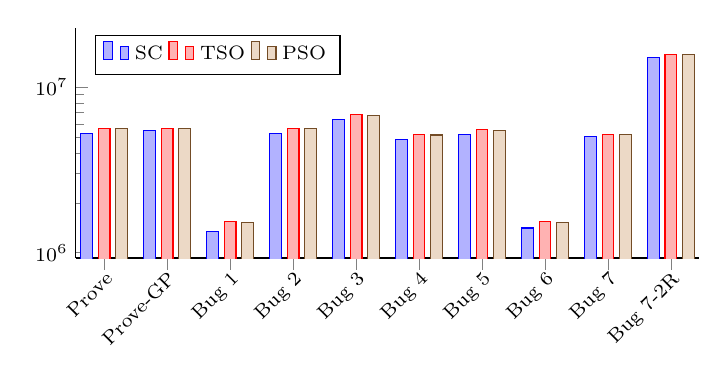
\begin{tikzpicture}
\scriptsize
\begin{axis}[
  ybar,
  bar width=0.15cm,
  height=4.5cm,
  width=9.5cm,
  axis lines*=left, % remove lines in the background
  ymode=log,
  %ylabel=Number of constraints,
  symbolic x coords={Prove, Prove-GP, Bug 1, Bug 2, Bug 3, 
                     Bug 4, Bug 5, Bug 6, Bug 7, Bug 7-2R,
                    },
  xtick=data,
  %nodes near coords, % numbers displayed above the bars
  %every node near coord/.append style={font=\small, rotate=90, anchor=west},
  xticklabel style={
    inner sep=0pt,
    anchor=north east,
    rotate=45
  },
  %enlargelimits=0.15,
  enlarge y limits=0.15, % space relative to the height of the plot
  enlarge x limits=0.05, % space relative to the width of the plot
  legend style={
    %anchor=north, at={(0.5, -0.9)}, % legend location
    legend pos=north west,
    legend columns=-1,
    font=\scriptsize},
]

\addplot % SC
  coordinates {(Prove, 5279600) (Prove-GP, 5476540)
               (Bug 1, 1343449) (Bug 2, 5279584) (Bug 3, 6374373)
               (Bug 4, 4847980) (Bug 5, 5161874) (Bug 6, 1410495)
               (Bug 7, 5022249) (Bug 7-2R, 15165557)
              };

\addplot % TSO 
  coordinates {(Prove, 5646959) (Prove-GP, 5646940)
               (Bug 1, 1540645) (Bug 2, 5646940) (Bug 3, 6805631)
               (Bug 4, 5170928) (Bug 5, 5522168) (Bug 6, 1541937)
               (Bug 7, 5201744) (Bug 7-2R, 15691102)
              };


\addplot % PSO
  coordinates {(Prove, 5617154) (Prove-GP, 5617135)
               (Bug 1, 1514657) (Bug 2, 5617135) (Bug 3, 6773763)
               (Bug 4, 5141123) (Bug 5, 5492607) (Bug 6, 1518307)
               (Bug 7, 5172720) (Bug 7-2R, 15647504)
              };

\legend{SC, TSO, PSO}
\end{axis}
\end{tikzpicture}
